\chapter{Anatomy of an extra-tropical cyclone}\label{Ch4}

% **************************** Define Graphics Path **************************
%\ifpdf
%    \graphicspath{{Chapter3/Figs/Raster/}{Chapter3/Figs/PDF/}{Chapter3/Figs/}}
%\else
%    \graphicspath{{Chapter3/Figs/Vector/}{Chapter3/Figs/}}
%\fi
\graphicspath{{Chapter3/Figs/}}


Many authors have emphasised the importance of shear (symmetric) instability in extra-tropical cyclones, namely in relation to precipitation bands. However, much of this work has been based on theory and little has been done to explore this mechanism in model forecasts. Here, I examine a single storm in a suite of model runs and compare results to theory.

\section{Aims}
\begin{itemize}
	\item Diagnose shear instability in a suite of model runs for an extra-tropical cyclone around 15th January 2004 over the Gulf Stream
	\item Explore the relationship of the shear instability with other variables, including precipitation
	\item Analyse atmospheric structure and characteristics that generate shear instability
	\item Examine differences between different model runs within same the resolution ensemble and also compare with members of different resolution
\end{itemize}

This storm on 15th January 2004 has been chosen as it has previously been used to show that the Gulf Stream is important \citep{sheldon2017warm}. 

%Total precipitation is comprised of convective precipitation and large scale (stratiform) precipitation. Convective precipitation produced by the convection scheme.


\section {Method}  \label{method}

Ensemble forecast hindcast data that is initialised on 12th January 2017 and set up with 12th January 2004 conditions was used. The vertical velocity data ($\omega$, Pa/s) is only complete at 12 hourly time steps and so the shear diagnostic could only be computed at 00 and 12 UTC. The storm developed over the Gulf Stream on 12 UTC 15th January, and so analysis is from initialisation + 4 days (96 hours).
%#, so expect the members to have diverged.
%
%Initial analysis based around establishing whether the shear instability seen in \cite{sheldon2017warm} in MetUM is also apparent in the ECMWF hindcast dataset. 
%
%Hindcast analysis is from the hindcast initialised on 00 UTC 12th January, so a lead time of at least +84 hours for the first time shown. Met Office was initialised 12 UTC 14th, so lead time of 24 hours only.


%Land mask

A spatial low pass and high pass filter was applied to the original data to obtain the small scale (${\omega}$', u', v') and mean ($\overline{w}$, $\overline{u}$, $\overline{v}$) values. An average over approximately 150 km in each direction for each point was calculated. Using 150 km allows for a low pass for ERA-Interim to be calculated, which is 0.75$^0$ resolution. The high pass, to capture the high frequency variability, was calculated by subtracting the low pass from the original field. This is to separate the low frequency background from the high frequency perturbations.
% which is comparable to the Met Office experiment \cite{sheldon2017warm}, where 120 km in each direction was used.

\begin{table}
	\caption{Low pass filter dimensions for different products}\label{t_lowpass}
	\begin{center}
		\begin{tabular}{cccc}
			%	\begin{tabular}{ | m{3.0cm} | m{2cm}| m{1.2cm} | m{2cm}| }
			\hline\hline
			Product & Resolution & No. grid points in each direction & Low pass scale \\
			\hline
			Hindcast & 0.2 & 7 & 140 km \\ 
			ERA-Interim & 0.75  & 2 & 150 km \\
			Forecast (2004) & 0.5 &  3 & 140 km \\ %%%%%%%%%% check			
			
			\hline
		\end{tabular}
	\end{center}
\end{table}


\begin{figure}
	\centering	
	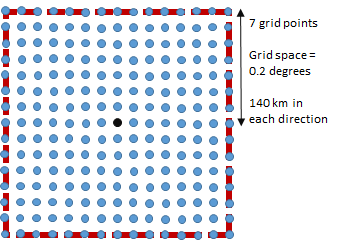
\includegraphics[width=16pc,angle=0]{low_pass.png}
	\caption{Domain used to create the low pass for the hindcast data.  The hindcast data is at 0.2 degree resolution and so the domain used is 1.4 degrees in each direction, approximately 140 km. At each grid point, all values within this domain are averaged to create the low pass at that point.}\label{fig:low_pass}
	\centering
\end{figure}

The shear diagnostic was computed using equation \ref{eq_diag} at the 500 hPa level.
%, which is comparable to the 5 km used in the Met Office analysis.

%The storm characteristics were different for the different members in term of location and intensity and so for each member, a rectangular domain around the storm minimum central pressure was computed, moving with the storm at each time step. The domain extends to the south and west of the low pressure centre, in order to capture the frontal activity?
%Histograms of variables within this domain were produced (number of datapoints).
%
%Other variables including precipitation, etc. also analysed using the same low pressure following domain.
%Eddy Kinetic energy also calculated and buoyancy diagnostic
%
%Table of diagnostics and other variables.
%
%The potential vorticity (PV) data in the ECMWF forecast hindcast is only available on the 320 isentropic level. 
%
%Analysis produced at the four main synoptic hours 00, 06, 12 and 18 UTC. They are the best gridded estimate of the state of the atmosphere (best fit to observations). 
%Forecast based on the 00/12 UTC Analysis. Meteorological parameters are written output for every forecast time step, 3-hourly intervals from 00 to 72 hours, and 6-hourly from 72 to 240 hours. Forecast 0 hr is same as analysis.

general stuff about preparing the data, interpolating levels?
Ensemble forecast hindcast data was used, with 'refdate' 12/01/2017, date of real-time forecast associated to re-forecast/hindcast, and 'hdate' 12/01/2004, base date of a hindcast. Initial analysis based around establishing whether the shear instability seen in (paper) in met office model is also apparent in the ECMWF hindcast dataset. 
The date of the following hindcast was 16/01/2007. The Met Office analysis ran from UTC 14/01/2004 and focussed on +24 hours, at ...
This analysis has a longer lead time (by 24 hours?) to the analysis time. At 12 UTC on 15th January, the storm had started to develop but was slower, less intense than the Met Office simulation. Therefore the main analysis time is 00UTC on 16th and the following two time steps.
The vertical velocity data ($\omega$, Pa/s) is only complete at 12 hourly time steps and so the diagnostic could only be computed at 00 and 12 UTC.


Land mask

\subsection {PV and momentum flux diagnostics}

The shear instability diagnostic:

\begin{equation} \label{eq_diag}
-\overline{w'u'} . \frac{\overline{\partial u}}{\partial z}
\end{equation}


% dubar/dp x (u'w')bar + dvbar/d[ x (v'w')bar
\begin{equation} \label{eq_diag1}
-\overline{w'u'} . \frac{\partial{\overline u}}{\partial z} + \overline{w'v'} . \frac{\partial{\overline v}}{\partial z}
\end{equation}

\begin{equation} \label{eq_diag2}
\frac{\partial}{\partial{t}} EKE = -\overline{w'u'} . \frac{\partial{\overline u}}{\partial z} + \overline{w'v'} . \frac{\partial{\overline v}}{\partial z} + ...
\end{equation}

NOTE: in calculating buoyancy, must take the low pass. This shows a mean spatial field. This is because it shows you that the small scale perturbations are having an effect on the large scale. If they evened out, the mean would be zero. This is also the case when take the low pass of the diagnostic.

% From Tellus warm path paper: To do so, we have applied spatial low-pass and high-pass filters on the 12 km grid (these were simply obtained by averaging at each point the 10 neighbouring points – separated by approximately 12 km so overall an average over 240 km – in the zonal and meridional directions, the ‘lowpass’, and then removing this average, the ‘high-pass’).  GIVES +120 in each direction for MO. I used +150 so that could do 2x0.75 for ERA

A spatial low pass and high pass filter was applied to the original data to obtain the prime' values (w', u', v') and bar values. An average over approximately 150 km in each direction for each point was calculated, which is comparable to the Met Office, where 120 km in each direction was used. In this case, using 150 km allows for a low pass for ERA-Interim to be calculated, which is 0.75 resolution. The high pass, to capture the high variability, was original minus low pass. This is to separate the low frequency background from the high frequency perturbations.


\begin{table}[h]
	\caption{Low pass filter dimensions for different products}\label{t_lowpass}
	\begin{center}
		\begin{tabular}{cccc}
			%	\begin{tabular}{ | m{3.0cm} | m{2cm}| m{1.2cm} | m{2cm}| }
			\hline\hline
			Product & Resolution & No. grid points in each direction & Low pass scale \\
			\hline
			Hindcast & 0.2 & 14 & 140 km \\ 
			ERA-Interim & 0.75  & 2 & 150 km \\
			Forecast & Variable &  x & x \\			
			
			\hline
		\end{tabular}
	\end{center}
\end{table}


\begin{figure}
	
	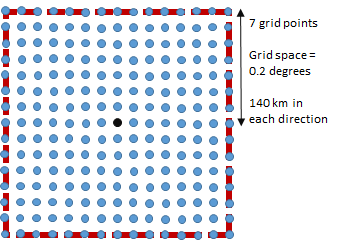
\includegraphics[width=16pc,angle=0]{low_pass.png}
	\caption{Domain used to create the low pass for the hindcast data.  The hindcast data is at 0.2 degree resolution and so the domain used is 1.4 degrees in each direction, approximately 140 km. At each grid point, all values within this domain are average to create the low pass at that point. ERA Interim has grid spacing f 0.75 degrees and so a low pass using 2 points in each direction was used (1.5 degrees). For the winter hindcast at 0.1 degree spacing, 14 grid points in each direction were used.}\label{fig:low_pass}
	\centering
\end{figure}


The 500 hPa level was analysed, which is comparable to the 5 km used in the Met Office analysis, and shear between levels used 600-400 hPa shear.

The storm characteristics were different for the different members in term of location and intensity and so for each member, a rectangular domain around the storm minimum central pressure was computed, moving with the storm at each time step. The domain extends to the south and west of the low pressure centre, in order to capture the frontal activity?
Histograms of variables within this domain were produced (number of datapoints).

Other variables including precipitation, etc. also analysed using the same low pressure following domain.
Eddy Kinetic energy also calculated:

\begin{equation} \label{eq_EKE}
\frac{\overline{(u'^{2}+v'^{2})}}{2} 
\end{equation}

The potential vorticity (PV) data in the ECMWF forecast hindcast is only available on the 320 isentropic level. 

Analysis produced at the four main synoptic hours 00, 06, 12 and 18 UTC. They are the best gridded estimate of the state of the atmosphere (best fit to observations). 
Forecast based on the 00/12 UTC Analysis. Meteorological parameters are written output for every forecast time step, 3-hourly intervals from 00 to 72 hours, and 6-hourly from 72 to 240 hours. Forecast 0 hr is same as analysis.

Pairs of ensemble members have the same SST field (member1\&6, member2\&7, member 3\&8, member 4\&9, member 5\&10)


\begin{figure}
	
	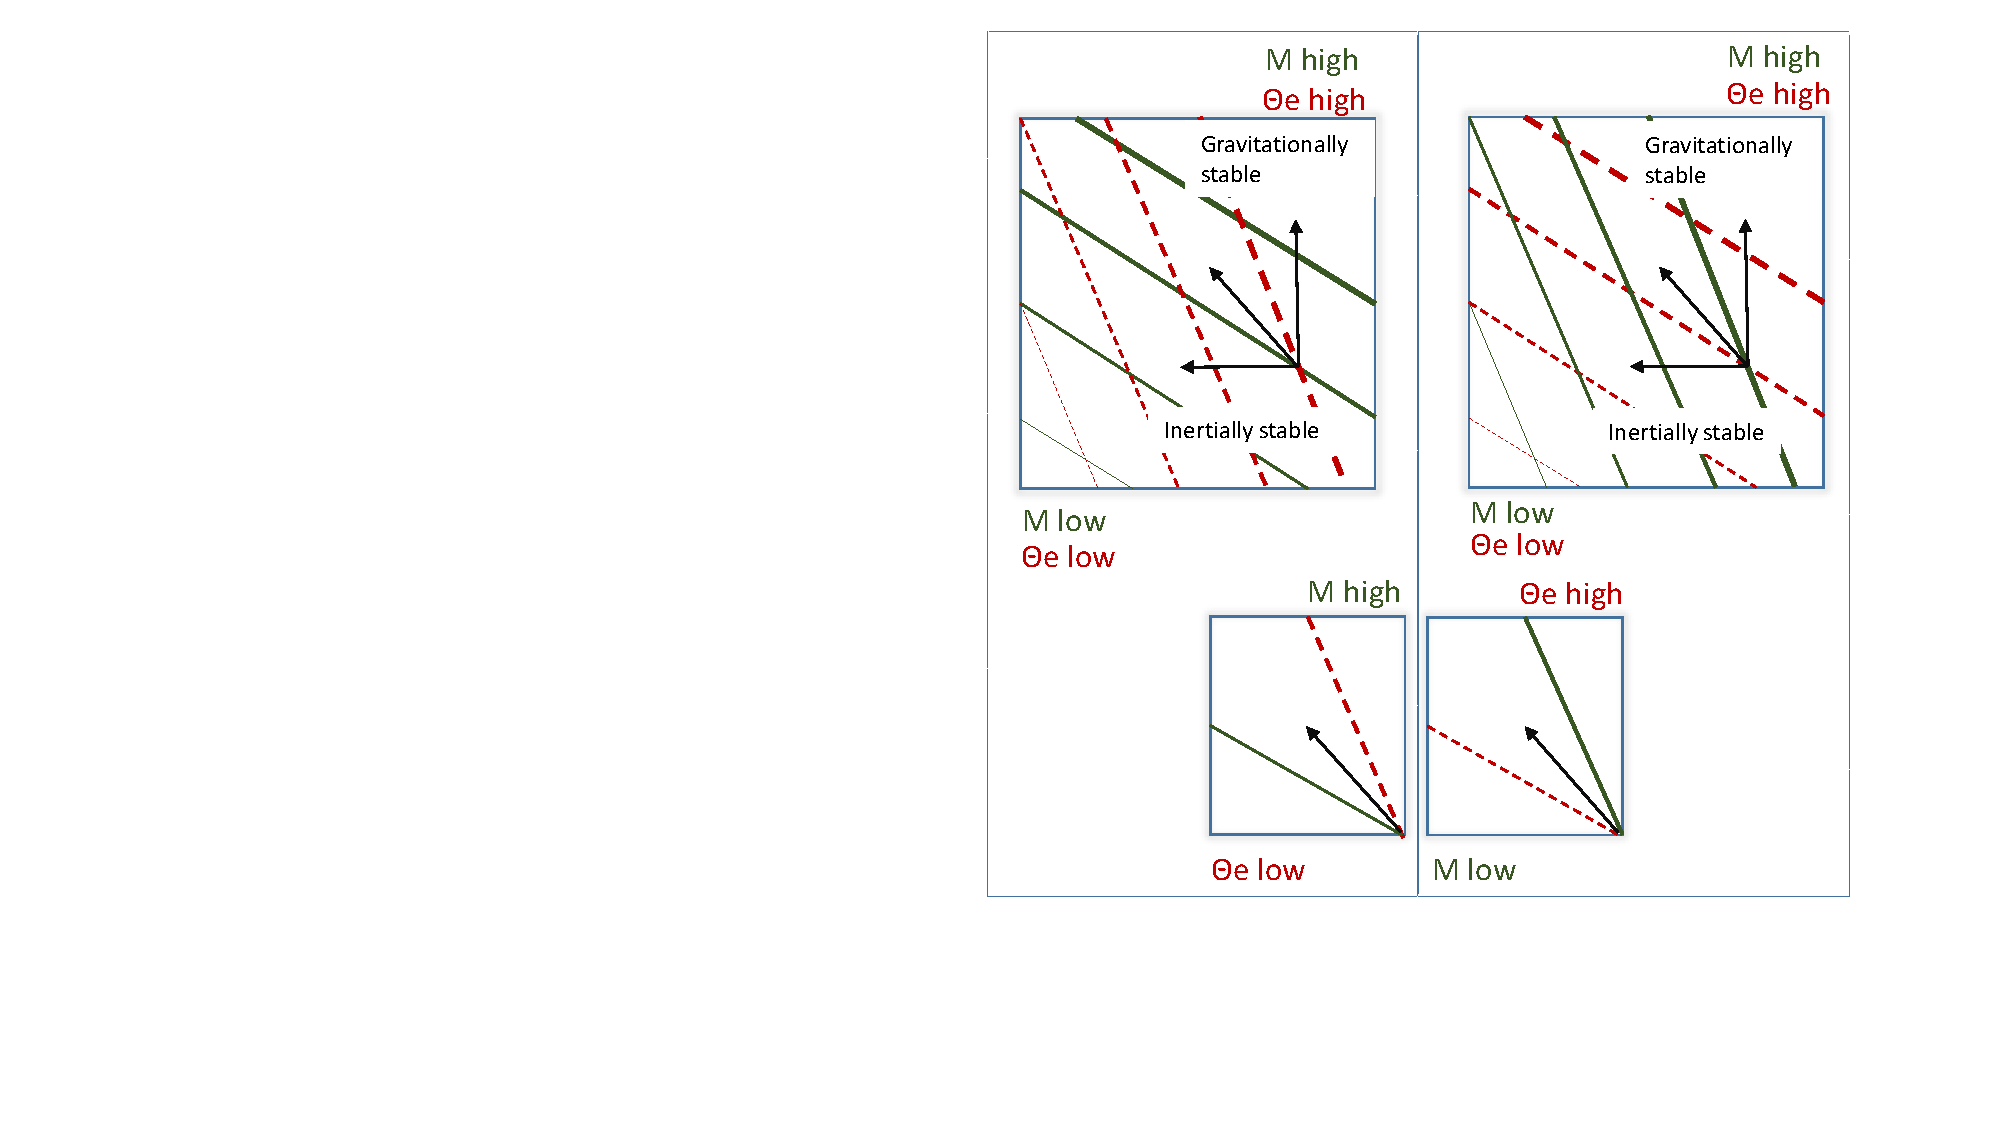
\includegraphics[width=38pc,angle=0]{mocrette_diagram.pdf}
	\caption{Symmetric instability. (what plane, ie x and z). Lines of constant equivalent potential temperature (theta e)  are shown in read dashed lines and lines of constant angular momentum (M) in solid green. Thickness of the lines increases towards  higher values. Both environments are baroclinic and theta e and M are low in the bottom left and high in the top right. The black arrows show direction of movement of air parcels. In both panels a and b, if a panel is moved to the left, it is inertially stable as it is moving towards an area of reduced angular momentum. Both panels, if a parcel is moved vertically, they are gravitationally stable as potential temperature is increasing. If an air parcel is moved along arrow x in a, it is moving towards lower potential temperature and high M, so . In the other case, it will move towards high theta e and low M, and so. Modified from \cite{morcrette2004radar}}\label{fig:symm_inst}
	\centering
\end{figure}


\begin{figure}
	
	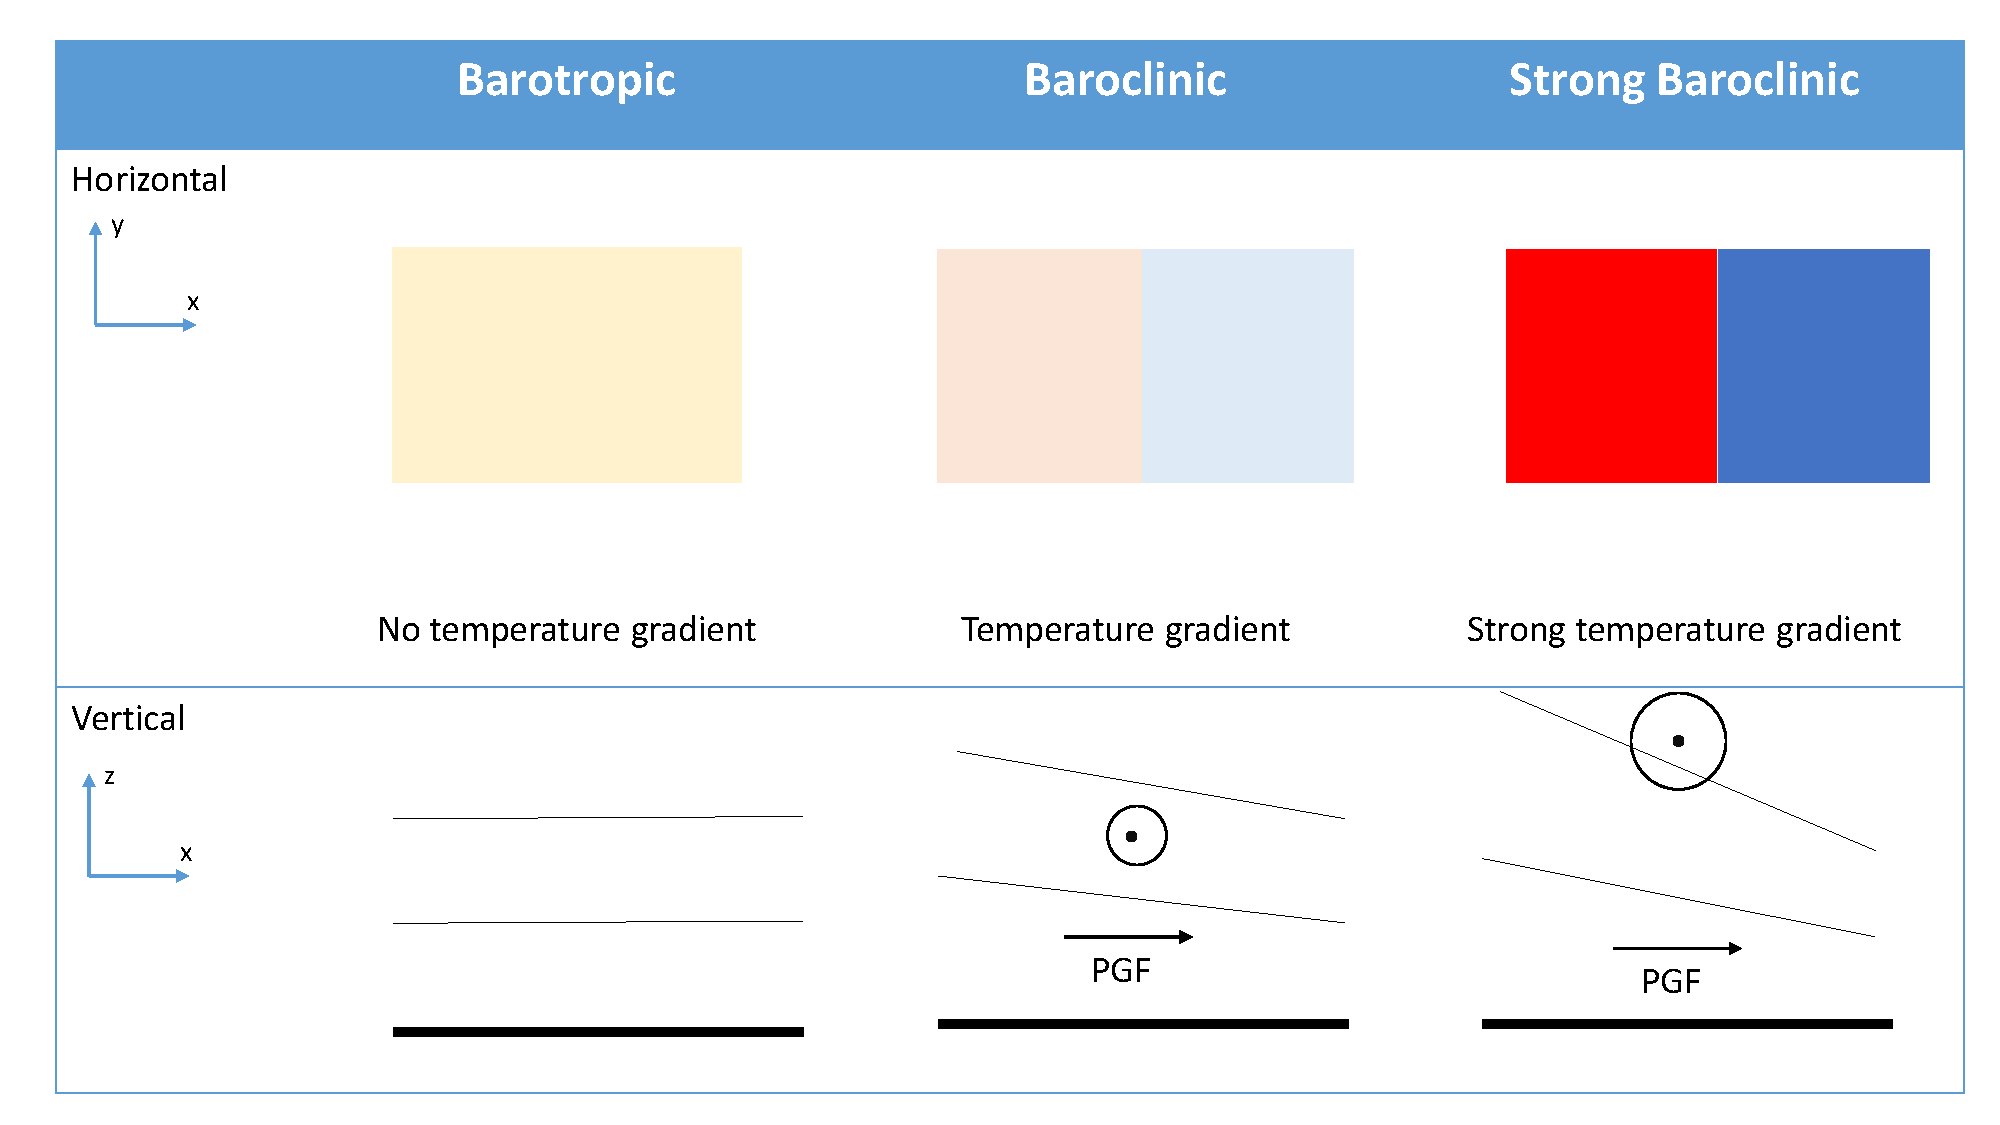
\includegraphics[width=34pc,angle=0]{barotropic2.pdf}
	\caption{Barotropic and baroclinic environments in the horizontal and vertical, and resultant pressure gradient force and thermal wind.}\label{fig:barotropic}
	\centering
\end{figure}

The high resolution single forecast was analysed for December 2016-February 2017. This is 9 km and downloaded on 0.1 degree resolution. Used 14 points for low pass

Buoyancy (b). g is acceleration due to gravity \(9.8ms^{-1}\). {\rho} is density.

\begin{equation} \label{eq_b}
b = -g\frac{\rho}{\rho_0}
\end{equation}

Total precipitation is comprised of convective precipitation and large scale (stratiform) precipitation. Convective precipitation produced by the convection scheme. 

Potential temperature is a more useful quantity than temperature as it is not affected my vertical movements - expansion and compression of air mass. Also most unstable path? requires no buoyancy. Calculated from temperature and pressure

% used to use the brackets and backslash. Now use equation environment \[\theta =  T \big(\frac{P_0}{P}) ^{0.286} \]
\begin{equation} \label{eq_theta}
\theta =  T \big(\frac{P_0}{P}) ^{0.286}
\end{equation}

Also calculated upright buoyancy (w'{\alpha})

\section{Results}

Results show analysis in the horizontal and vertical of a single extra-tropical cyclone from 15th January 12 UTC to 17th January 00 UTC. 

\subsection{Analysis in latitude/longitude plane}

\begin{figure}
	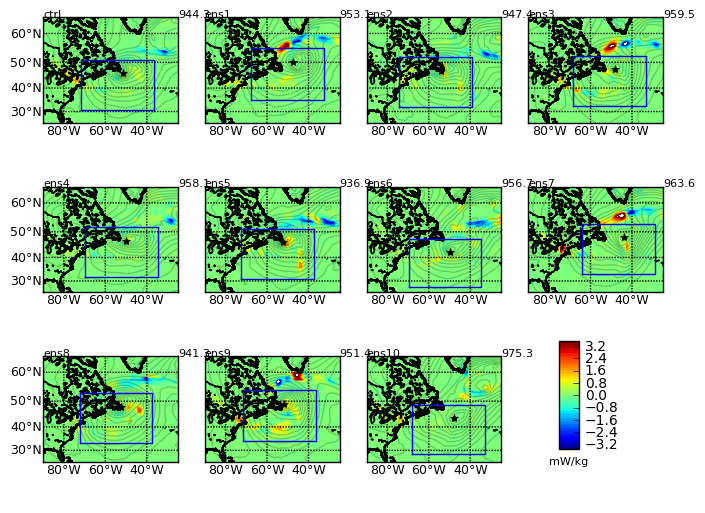
\includegraphics[width=42pc,angle=0]{plot_var_poly_all_diag500_msl_00UTC_17.png} % Y:/Code_Data/Chapter2_3/Plots/Jan04_storm/HC_120104/
	\caption{Mean sea level pressure (contours) and shear diagnostic (filled contours) for all hindcast members at 00 UTC 17th January 2004. The centre of this low pressure system is marked with a *. The member name is given on the top left of the plot and the minimum pressure on the top right (in hPa). }\label{fig:HC_all}
\end{figure}

Figure \ref{fig:HC_all} shows the shear diagnostic and mean sea level pressure contours at 00 UTC on 17th January (+114 hours) in the hindcast control and 10 members. All of the runs simulate a cyclone, but with different characteristics, for example minimum central pressure and location. The shear diagnostic is resolved in all of the runs, although there are large differences in intensity. The shear diagnostic is generally associated with fronts, which mark the boundary of warm and cold air masses within with the cyclone. Such fronts can be identified by kinks in the isobars and also temperature analysis, with warm air behind the warm front and cold air behind the cold front, with a steep gradient in temperature observed at each front.

The following analysis focusses on ensemble member 9, as this run exhibits a relatively strong diagnostic, which is aligned in such a way that makes it suitable for cross-section analysis (section \ref{cx_analysis}).

\begin{figure}[h]
	\centering
	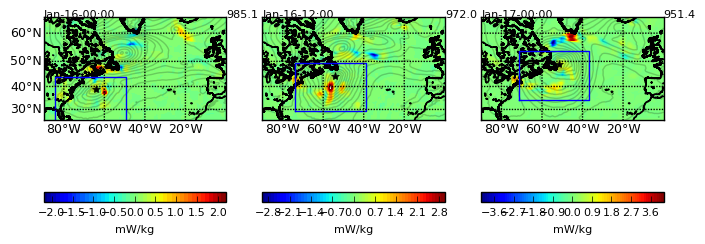
\includegraphics[width=34pc,angle=0]{plot_var_poly_ens9_diag500_msl_12UTC_15_3cb.png} % Y:/Code_Data/Chapter2_3/Plots/Jan04_storm/HC_120104/
	\caption{Mean sea level pressure (contours) and diagnostic (filled contours) for hindcast ensemble member 9 at 12 UTC 15th, 00 UTC 16th, 12 UTC 16th January 2004.The centre of this low pressure system is marked with a *. The time is on the top left of the plot and the minimum pressure on the top right (in hPa)}\label{fig:HC_ens9}
	\centering
\end{figure}

Figure \ref{fig:HC_ens9} shows the evolution of ensemble 9 from 00 UTC 16th, with 12-hourly time steps. As the storm deepens and moves north-eastwards, the shear diagnostic increases in intensity. The shear diagnostic also follows the regions of strong gradient in potential temperature, as seen in figure \ref{fig:HC_ens9_pt_RH_precip}, marking cold and warm fronts. Figure \ref{fig:HC_ens9_pt_RH_precip} also shows relative humidity at 500 hPa and precipitation for the 12 hours centred on the time. Moist air is present in the warm sector and the the cold air advected in behind the cold front is relatively dry. The precipitation is intense in the storm centre and along the fronts, especially the trailing cold front, where the sinking cold air is forcing the moist, warm air to ascend.


\begin{figure}	%%% remove [h] here and plots fell into place
	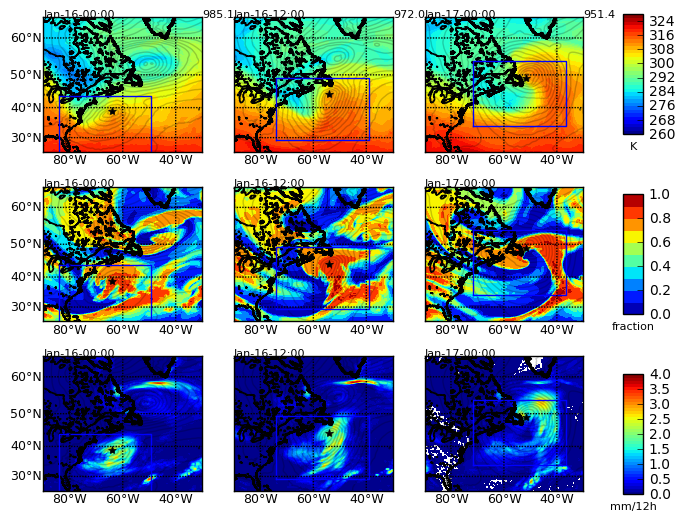
\includegraphics[width=36pc,angle=0]{plot_var_poly_ens9_ptRHprecip_12UTC_15.png} % Y:/Code_Data/Chapter2_3/Plots/Jan04_storm/HC_120104/
	\caption{Filled contours: Top panels: 500 hPa potential temperature. Middle panels: 500 hPa relative humidity. Bottom panels: 12-hour precipitation centred on time. Mean sea level pressure is shown in contour line. Hindcast ensemble member 9 at 12 UTC 15th, 00 UTC 16th, 12 UTC 16th January 2004. The centre of this low pressure system is marked with a *. The time is on the top left of the plot and the minimum pressure on the top right (in hPa)}\label{fig:HC_ens9_pt_RH_precip}
	\centering
\end{figure}


%Plots of diag with precip contours overlaid
%\begin{figure}	[h]
%	\includegraphics[width=28pc,angle=0]{Y:/Code_Data/Chapter2_3/Plots/Jan04_storm/HC_120104/plot_var_poly_ens9_diag_precip_12UTC_15.png}
%	\caption{Diagnostic and precip 12 UTC 16th ens9}\label{fig:HC_diag_precip}
%	\centering
%\end{figure}

These results from the hindcast are compared to the coarser ERA-Interim analysis at the same time. The low pass of ERA-Interim was calculated using just two grid points in each direction, as the spacing is much coarser at 0.75 degrees. The shear diagnostic for this same storm is shown in figure \ref{fig:ERA_diag}. The scale is an order of magnitude smaller than figure \ref{fig:HC_ens9}, where hindcast members were 0.2 degrees resolution. During these three time steps, the minimum central pressure is deeper in ERA-Interim than the hindcast ensemble member 9 (970, 952, 948 compared to 985, 972, 951 hPa). However, this is likely due to the timing of the storm system and the higher resolution hindcast member is deepening at a faster rate than the ERA-Interim run. The variables in figure \ref{fig:ERA_pt_RH_precip} show similar characteristics to that for ensemble member 9, although the precipitation is not as intense.


\begin{figure}
	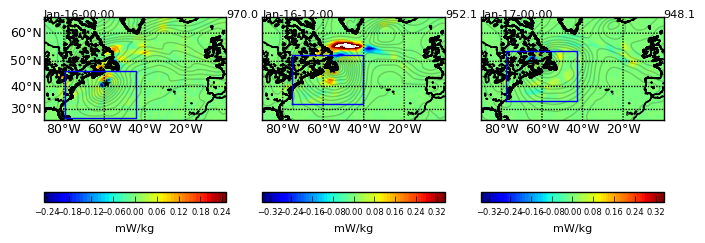
\includegraphics[width=36pc,angle=0]{plot_var_poly_ERA_diag500_msl_12UTC_15.png} % Y:/Code_Data/Chapter2_3/Plots/Jan04_storm/ERA/
	\caption{Mean sea level pressure (contours) and diagnostic (filled contours) for ERA-Interim at 12 UTC 15th, 00 UTC 16th, 12 UTC 16th January 2004.The centre of this low pressure system is marked with a *. The time is on the top left of the plot and the minimum pressure on the top right (in hPa)}\label{fig:ERA_diag}
	\centering
\end{figure}

\begin{figure}	%%% remove [h] here and plots fell into place
	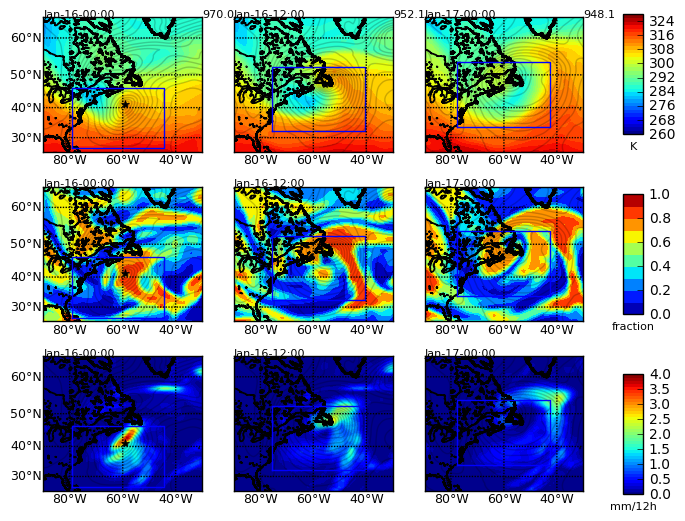
\includegraphics[width=36pc,angle=0]{plot_var_poly_ERA_ptRHprecip_12UTC_15.png}
	\caption{Filled contours: Top panels: 500 hPa potential temperature. Middle panels: 500 hPa relative humidity. Bottom panels: 12-hour precipitation centred on time. Mean sea level pressure is shown in contour line. ERA-Interim at 12 UTC 15th, 00 UTC 16th, 12 UTC 16th January 2004. The centre of this low pressure system is marked with a *. The time is on the top left of the plot and the minimum pressure on the top right (in hPa)}\label{fig:ERA_pt_RH_precip}
	\centering
\end{figure}

In 2004, the deterministic forecast member was at 0.5$^0$ degree resolution and so 3 grid points were used to create the low pass. Here (figure \ref{fig:fc_diag}), the shear diagnostic is larger than that in ERA-Interim, but smaller than that in the finer hindcast members. This storm has the lowest central pressure at each time step compared to ensemble member 9 and ERA-Interim, but this is likely to be due to the storm being approximately 12 hours ahead of the hindcast run. The precipitation in this single forecast member is more intense than that in ensemble member 9 and ERA-Interim.

\begin{figure}
	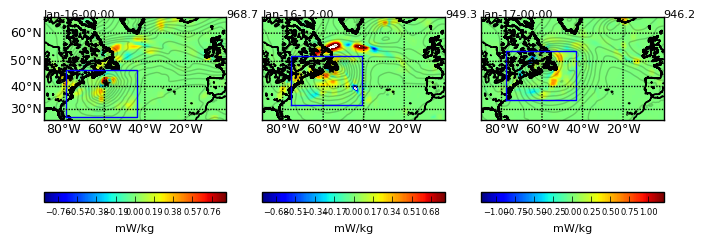
\includegraphics[width=34pc,angle=0]{plot_var_poly_fc_diag500_msl_12UTC_15.png} % Y:/Code_Data/Chapter2_3/Plots/Jan04_storm/FC_140104/
	\caption{Mean sea level pressure (contours) and diagnostic (filled contours) for operational forecast at 12 UTC 15th, 00 UTC 16th, 12 UTC 16th January 2004.The centre of this low pressure system is marked with a *. The time is on the top left of the plot and the minimum pressure on the top right (in hPa)}\label{fig:fc_diag}
	\centering
\end{figure}

\begin{figure}	%%% remove [h] here and plots fell into place
	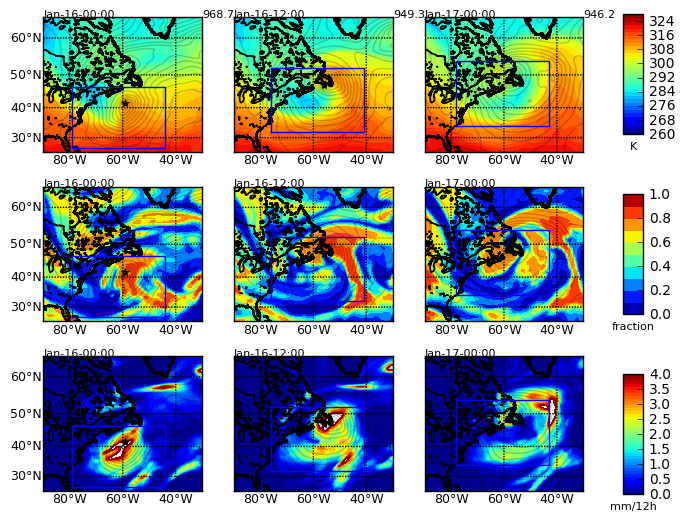
\includegraphics[width=36pc,angle=0]{plot_var_poly_fc_ptRHprecip_12UTC_15.png}
	\caption{Filled contours: Top panels: 500 hPa potential temperature. Middle panels: 500 hPa relative humidity. Bottom panels: 12-hour precipitation centred on time. Mean sea level pressure is shown in contour line. Operational forecast at 12 UTC 15th, 00 UTC 16th, 12 UTC 16th January 2004. The centre of this low pressure system is marked with a *. The time is on the top left of the plot and the minimum pressure on the top right (in hPa)}\label{fig:fc_pt_RH_precip}
	\centering
\end{figure}


These results suggest that with a high resolution model is required to resolve this shear instability. 

%PV from ERA and forecast
%Moist entrpoy


\subsection{Analysis in vertical cross-sections} \label{cx_analysis}

The following section shows vertical cross section analysis for ensemble member 9. The wind bars are calculated by taking the horizontal wind speed (m/s) and integrating this for an hour. The coloured contours show relative humdity and contour lines show potential temperature. The two line graphs show the shear diagnostic with height and horizontal distance (at 500 hPa), and precipitation is also shown in the horizontal plane. The original data did not include information on 600 hPa, so all values on this level are interpolated. The contours have data on 9 level (200, 300, 400, 500, 600, 700, 850, 925, 1000 hPa) and values in between are calculated by the plotting function.

% by multiplying by 3600 so give a horizontal distance each individual air parcel has moved. Metres into degrees by dividing by 110540. Plot the bar from start latitude to end latitude. Vertical movement, multiply omega (Pa/s) by 3600 and divide by 100 to get hPa/hour. Plot the line between the two start points and the two end points.

\begin{figure}[h]	
	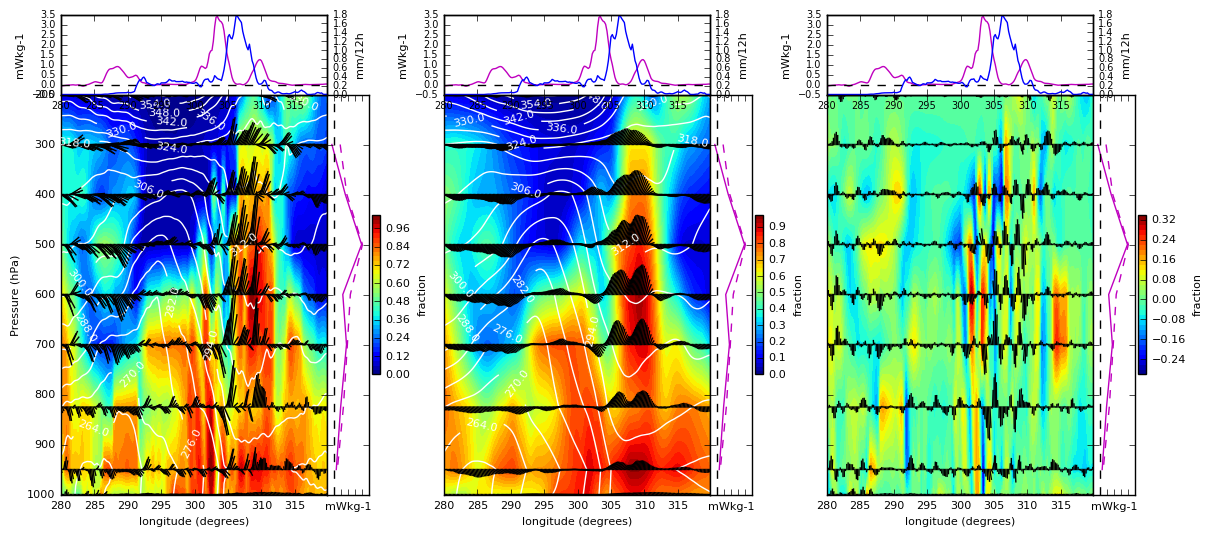
\includegraphics[width=40pc,angle=0]{cx3_sub_u_RH_pt_ens9_40N_12UTC_16th.png} % Y:/Code_Data/Chapter2_3/Plots/Jan04_storm/HC_120104/
	\caption{Vertical cross-section on 12 UTC 16th at 40N. Relative humidity is shown in filled contours and isentropes are shown in white contour lines. Wind bars are calculated using zonal (u) and vertical ($\omega$) winds. The left hand plot shows the original data. The middle plot shows the low pass (wind bars, filled contours and contour lines), and the right hand plot shows the high pass (wind bars and filled contour lines). The horizontal line plots show the shear diagnostic in magenta and 12-hourly precipitation (mm) in blue. The vertical line plots show the mean diagnostic (solid magenta) and mean absolute diagnostic (dashed magenta).}\label{fig:HC_cxA}
	\centering
\end{figure}

At 12UTC 16th January (figure \ref{fig:HC_ens9}), the cold front is aligned north-south and a vertical cross-section at 40N is plotted to see the vertical motion and atmospheric characteristics across this front (figure \ref{fig:HC_cxA}). The wind bars show vertical motion throughout the depth of the troposphere, associated with a region of high relative humidity and high potential temperature. This ascent is in the warm, moist air in the warm sector of the cyclone, as the colder air behind the cold front undercuts this air mass and forces its ascent. The highest values of the shear instability diagnostic are seen in this region of high relative humidity and peak at 500 hPa. The precipitation peaks just to the west of this region, where there is a strong gradient in potential temperature. There is a second, smaller precipitation peak further west, just past the peak in the shear diagnostic.

%This descending air is also seen in the original and low pass wind bars.
%At 40N seems most intense. Also took sections at 38N and 42N and same pattern shown.
%Moist entropy only valid where saturated

%\begin{figure}[h]	
%	\includegraphics[width=40pc,angle=0]{Y:/Code_Data/Chapter2_3/Plots/Jan04_storm/HC_120104/cx3_sub_u_s_pt_ens9_40N_12UTC_16th.png}
%	\caption{Vertical cross-section 12 UTC 16th. s filled contours. pottemp and u 40N}\label{fig:HC_cxB}
%	\centering
%\end{figure}

%Cold front analysis - second time step, EW oriented - look at 38 or 39 N
%
%
\begin{figure}[h]	
	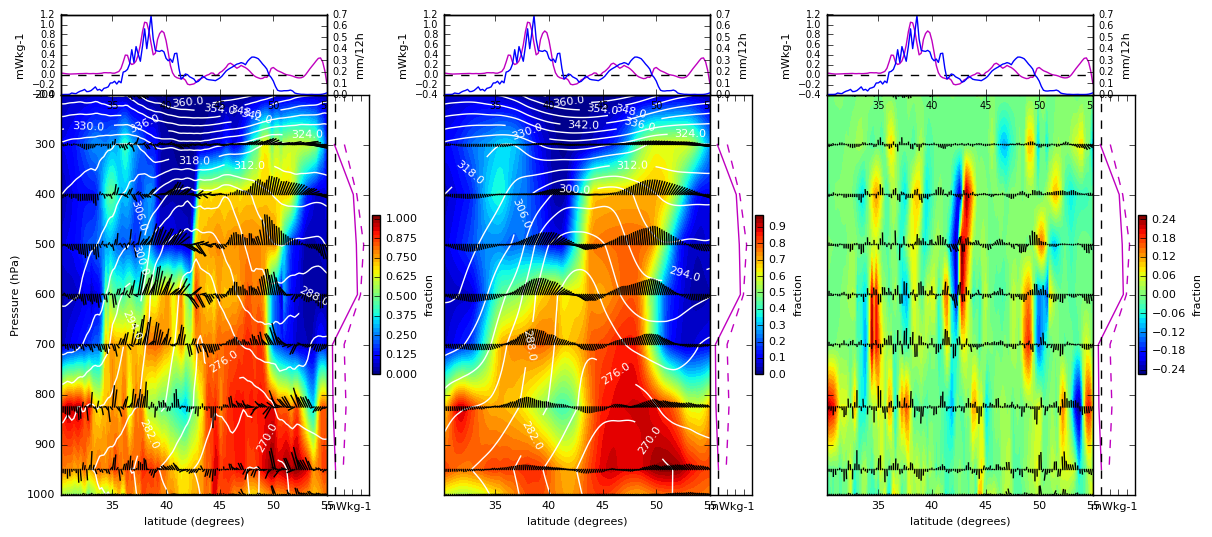
\includegraphics[width=40pc,angle=0]{cx3_sub_v_RH_pt_ens9_56W_00UTC_17th.png}
	\caption{Vertical cross-section on 00 UTC 17th at 56W. Relative humidity is shown in filled contours and isentropes are shown in white contour lines. Wind bars are calculated using meridional (v) and vertical ($\omega$) winds. The left hand plot shows the original data. The middle plot shows the low pass (wind bars, filled contours and contour lines), and the right hand plot shows the high pass (wind bars and filled contour lines). The horizontal line plots show the shear diagnostic in magenta and 12-hourly precipitation (mm) in blue. The vertical line plots show the mean diagnostic (solid magenta) and mean absolute diagnostic (dashed magenta).}\label{fig:HC_cxC}
	\centering
\end{figure}

Twelve hours later, at 00 UTC on 17th January, this cold front has changed position as the storm has evolved and is oriented east-west at around 36N to 40N. A section at 56W is taken and the v wind bars are plotted on a latitudinal plane (figure \ref{fig:HC_cxC}). The shear diagnostic is largest from 600 to 400 hPa, where there are large relative humidity values and ascent.


%\begin{figure}[h]	
%	\includegraphics[width=40pc,angle=0]{Y:/Code_Data/Chapter2_3/Plots/Jan04_storm/HC_120104/cx3_sub_v_s_pt_ens9_58W_00UTC_17th.png}
%	\caption{Vertical cross-section 00 UTC 17th. RH and v 58W}\label{fig:HC_cxC}
%	\centering
%\end{figure}

At 00 UTC on 17th and at approximately 52N, the warm front is aligned east-west if a section is taken at 45W. The warm front can be seen by the dip in the isentropes and this is in line with the peak in relative humidity and also two peaks in shear instability at 500 hPa.

\begin{figure}[h]	
	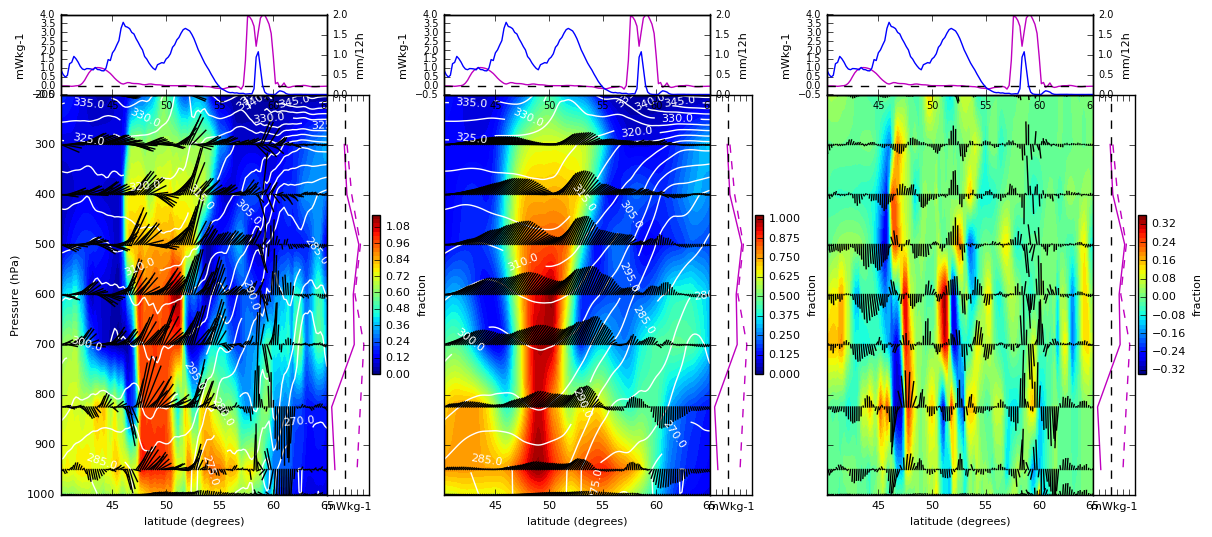
\includegraphics[width=40pc,angle=0]{cx3_sub_v_RH_pt_ens9_45W_00UTC_17th.png}
	\caption{Vertical cross-section on 00 UTC 17th at 45W. Relative humidity is shown in filled contours and isentropes are shown in white contour lines. Wind bars are calculated using meridional (v) and vertical ($\omega$) winds. The left hand plot shows the original data. The middle plot shows the low pass (wind bars, filled contours and contour lines), and the right hand plot shows the high pass (wind bars and filled contour lines). The horizontal line plots show the shear diagnostic in magenta and 12-hourly precipitation (mm) in blue. The vertical line plots show the mean diagnostic (solid magenta) and mean absolute diagnostic (dashed magenta).}\label{fig:HC_cxE}
	\centering
\end{figure}

%
%Through low pressure centre - capture some wf and some cf
%
%%\begin{figure}[h]	
%%	\includegraphics[width=40pc,angle=0]{Y:/Code_Data/Chapter2_3/Plots/Jan04_storm/HC_120104/cx3_sub_v_s_pt_ens9_52W_00UTC_17th.png}
%%	\caption{Vertical cross-section 00 UTC 17th. pottemp and v 57.4N}\label{fig:HC_cxF}
%%	\centering
%%\end{figure}
%
%\begin{figure}[h]	
%	\includegraphics[width=40pc,angle=0]{Y:/Code_Data/Chapter2_3/Plots/Jan04_storm/HC_120104/cx3_sub_v_RH_pt_ens9_52W_00UTC_17th.png}
%	\caption{Vertical cross-section 00 UTC 17th. pottemp and v 59N}\label{fig:HC_cxG}
%	\centering
%\end{figure}

%
%\subsection{Correlation analysis}
%
%%%%%%%%%%%%%%%%%%%%%%% SCATTER PLOTS %%%%%%%%%%%%%%%%%%%%%%%%%%%%
%Include all members and ERA and fc and MO amplitude of diagnostic. See a linear trend in terms of resolution and diagnostic strength?
%When do you reach the maximum strength? What is physically possible? asymptote?
%
%Talk about box following storm. Or just do over entire region, 1D correlation.
%%\begin{figure}
%	
%	\includegraphics[width=34pc,angle=0]{Y:/Code_Data/Chapter2_3/Plots/Jan04_storm/HC_120104/plot_var_poly_ctrl_diag500_msl_12UTC_15_3cb.png}
%	\caption{Mean sea level pressure (contours) and diagnostic (filled contours) for hindcast control at 12 UTC 15th, 00 UTC 16th, 12 UTC 16th January 2004.}\label{fig:HC_ctrl}
%	\centering
%\end{figure}

%Perhaps differences between ensembles because had previous storm that affected the path of this next storm

%Plots with SST contours?


These results have so far shown that shear instability can be resolved in all of the model simulations examined, although an increase in intensity is shown with an increase in resolution. This instability is strongly associated with the warm and cold fronts in the extra-tropical cyclone, with ascent seen throughout the depth of the troposphere. The instability peaks at around 500 hPa, which is consistent with other studies. Just one ensemble member from the 11-member hindcast has been presented here. However, large differences in storm characteristics can be seen between the different ensemble members.


\section {Future work}  

I hope to examine in more detail the relationship between the shear instability diagnostic and precipitation bands. I also aim to explore further the spread between the ensemble members. This work focussing on a single storm and the dynamics associated with this instability is important for setting up the work in the following chapter, where a climatology of storms will be analysed.



\section{Conclusions}
%Include limitations







\section{Estimate the impact of the new mechanism on the climatological mean state of the North Atlantic}

\subsection{ Hypothesis / Aim}
Develop a simple theoretical model of the findings in Part 1 and 2



%\begin{figure}	
%	\includegraphics[width=34pc,angle=0]{Y:/Code_Data/Plots_new/ECMWF/120104_maps/calcs/masksq_poly_time_diag-precip-msl_ens9_12012004.pdf}
%	\caption{Data}\label{fig:data}
%	\centering
%\end{figure}


%I will assess whether or not the warm path mechanism (Section 3.3), examined in the Met Office case study \cite{sheldon2017warm} and in section \ref{Ch2}, has relevance to the climatological state of the storm-track in the North Atlantic

I will examine the relationship between cyclone activity in the North Atlantic and the sea surface temperature in the Gulf Stream region. I will also estimate the impact of shear instability and slantwise convection on the climatological mean state of the North Atlantic. It is well established that many forecast busts over Europe are due to poor representation of atmospheric blocking \cite{rodwell2013characteristics}. It is also known that blocking and the state of the North Atlantic Oscillation (NAO) are related to storm track activity \citep{vallis2008local}. In this study, I propose that the small-scale mechanism of shear instability is a missing process in climate models, which can have a detrimental effect on the downstream forecast.

%
%Recent numerical experiments with high horizontal resolution (grid spacing of 25km or less) have suggested that the impact of the Gulf Stream on the “storm track” is mediated by the frontal circulation embedded in extra-tropical cyclones. In a series of controlled experiments with the UK Met Office Model, we were able to show that the frontal circulation can be destabilized by the Gulf Stream, with associated injection of low potential vorticity air at upper levels and a potential impact on blocking events further downstream, but we could not assess whether this effect was systematic (Sheldon et al., 2017). In this work, we address this issue by analysing an 11-member ensemble hindcast from ECMWF over the period 2007-2017 at a horizontal resolution of 16km. A large spread is found amongst ensemble members suggesting that, rather than systematically affecting the frontal circulation of cyclones, the effect of the Gulf Stream on them has to be understood within a statistical framework. 

\section{Aims}
\begin{itemize}
	\item Analyse operational forecasts, ensemble hindcasts and reanalysis run at ECMWF (1996 to present) using the shear instability diagnostic
	\item Explore the relationship between shear instability and state of the Gulf Stream
	\item Determine the impact of shear instability in extra-tropical cyclones on the downstream weather over western Europe
	\item Examine the upstream storm track activity (and shear instability) associated with forecast busts in terms of blocking indices
\end{itemize}


%Gerber and Valis 2009

%Unlike upright convection, slantwise convection transports air from low levels at one latitude to high levels at a different latitude. 

% http://www.atmo.arizona.edu/students/courselinks/spring16/atmo541b/handouts/pv_climo_bluestein1992.png

%\begin{figure}[h]
%	\centering
%	\noindent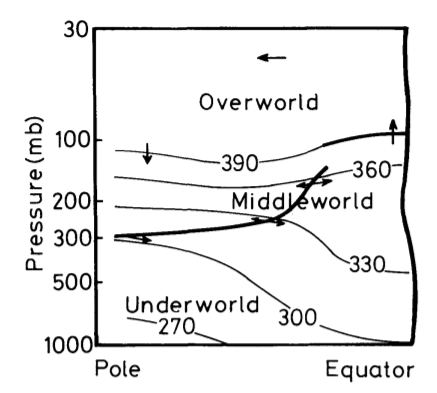
\includegraphics[width=18pc]{H:/Documents/Thesis/phd-thesis-template-2.2.2_AC/phd-thesis-template-2.2.2/Figs/Hoskins_PVview.png}
%	\caption{A schematic view of potential vorticity in the atmosphere. Isentropes every 30 K marked. Tropopause in thick black line. (what PV value?). The arrow indicate some boundaries. The equatorial boundary is defined by the zero PV contour. Source: \cite{hoskins1991towards}} \label{fig:PV_profile}
%\end{figure}

%Time series data downloaded 4th Oct https://www.esrl.noaa.gov/psd/gcos_wgsp/Timeseries/NAO/
%East Atlantic from http://www.cpc.ncep.noaa.gov/data/teledoc/ea.shtml
%Gulf Stream northern wall from PML http://www.pml-gulfstream.org.uk/data.htm

I will analyse hindcasts from 1996-2017 for DJF only. This data will come from hindcasts run on 26 dates (table \ref{t_winterdates}). To focus on the highest resolution sections of these runs (0.2$^0$), I will just retain the first 15 days.

\begin{table}[h]
	\caption{DJF hindcast dates 2016-2017. A total of 26 hindcast dates}\label{t_winterdates}
	\begin{center}
		\begin{tabular}{c}
			%	\begin{tabular}{cc}
			\hline\hline
			Mondays \\
			05/12, 12/12, 19/12, 26/12, 02/01, 09/01, 16/01, 23/01, 30/01, 06/02, 13/02, 20/02, 27/02 \\ 
			\hline
			Thursdays \\			
			01/12, 08/12, 15/12, 22/12, 29/12, 05/01, 12/01, 19/01, 26/01, 02/02, 09/02, 16/02, 23/02  \\ 			
			\hline
		\end{tabular}
	\end{center}
\end{table}

%There are 31 times and 20 years and levels 400, 500, 700. Interpolate to get level 600.
Figure \ref{t_winter_timeline} illustrates the many runs that will be analysed. At times there will be runs initialised on 5 different dates that are representing the same time, which will give 55 ensemble members.

\
As well as the ensemble hindcasts that are at 0.2$^0$ resolution, I will also analyse the operational control forecast, which has a different resolution depending on the year (see table \ref{t_ecmwf2}) along with the ERA-Interim renanalysis.
Using such a rich sample allows for both the climatology over a long time period to be examined, and also 
the ensemble spread on shorter timescales.


\section{Method}
Work has begun on downloading the large datasets required. I have also developed a working code for diagnosing atmospheric blocking based on the below.


\subsection{Atmospheric blocking indices}

A blocking time series has been calculated based on the method by \cite{davini2016northern}. To examine blocking over the Euro-Atlantic region, 60W-22.5W is the West Atlantic and 22.5W-45E is the East Atlantic.

$\phi_{0}$ = 60N; $\phi_{S}$ = 41.25N; $\phi_{N}$ = 78.75N; $\Delta$ = -3.75, 0, 3.75

\begin{equation} \label{eqblock1} %%% did not like blank line below - displaymath needs $$
GHGS(\lambda_{0}, \Delta) = \frac{Z500(\lambda_{0}, \phi_{0}+ \Delta) - Z500(\lambda_{0}, \phi_{S}+ \Delta)}
{\phi_{0} - \phi_{S}}
\end{equation}

\begin{equation} \label{eqblock2}
GHGN(\lambda_{0}, \Delta) = \frac{Z500(\lambda_{0}, \phi_{N}+ \Delta) - Z500(\lambda_{0}, \phi_{0}+ \Delta)}
{\phi_{N} - \phi_{0}}
\end{equation}


\begin{equation} \label{eqblock3}
IB(\lambda_{0}) = 1,   \textbf{if for any} \Delta ,  GHGS(\lambda_{0}, \Delta) > 0  , \textbf{and},   GHGN(\lambda_{0}, \Delta) < -5 m 
\end{equation}


This method, like many similar calculate the gradient in geopotential height (z) in a southern and northern region. If the gradient in the southern part is positive (i.e. increased westerlies) and in the northern part is negative (decreased westerlies), then blocking is diagnosed.
%Why 500 hPa?

% http://www.metoffice.gov.uk/learning/learn-about-the-weather/how-weather-works/factors-that-influence-uk-winters

%\begin{figure}[h]
%	\centering
%	\noindent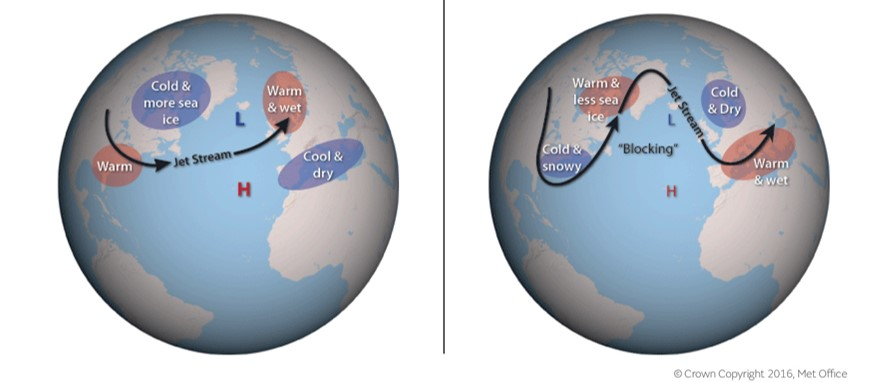
\includegraphics[width=38pc]{H:/Documents/Thesis/phd-thesis-template-2.2.2_AC/phd-thesis-template-2.2.2/Figs/nao_mo.jpg}
%	\caption{NAO}\label{fig:NAO}
%\end{figure}

A sector is considered blocked if at least 11.25 degrees in longitude is consistently blocked. A blocking event requires persistence in time of at least five consecutive days. Figure \ref{fig:block_criteria} shows the GHGS values for 2015. The red box in the bottom left hand corner illustrates the dimensions in time and space that must be satisfied in order for a blocking event to be categorised.
%NB Update plot to plot Hov of combined GHGS A and GHGNA???

%\begin{figure}	
%	\includegraphics[width=22pc,angle=0]{Y:/Code_Data/Chapter2_3/Plots/final/Hovm_GHGNA_2015_area.png}	
%	\caption{Blocking event criteria in space and time}\label{fig:block_criteria}
%	\centering
%\end{figure}

%This blocking index has been calculated using... forecast ? hindcast?

%\begin{figure}
%		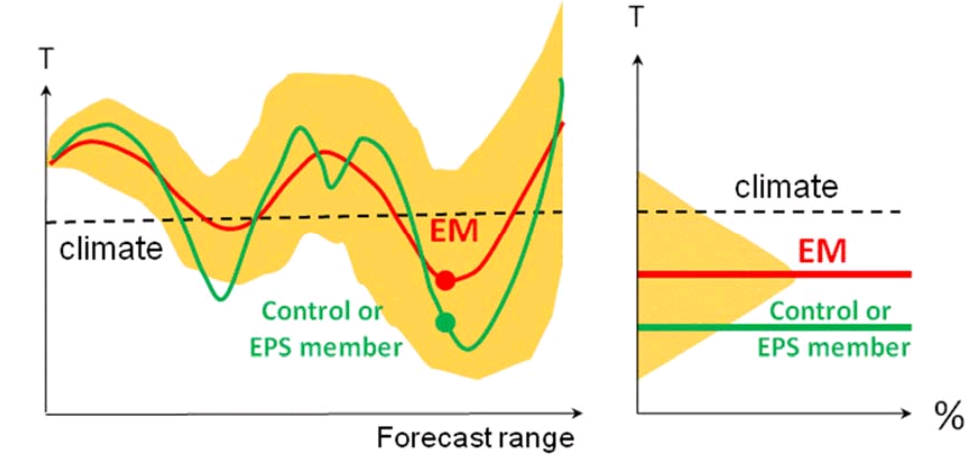
\includegraphics[width=22pc,angle=0]{H:/Documents/Thesis/phd-thesis-template-2.2.2_AC/phd-thesis-template-2.2.2/Figs/ens_spread.png}
%	\caption{Blocking events from ...}\label{fig:block_events}
%	\centering
%\end{figure}

%The period being examined initially is 2008-2017 DJF. 



\section{Possible future analysis across thesis chapters 2 and 3}

% https://software.ecmwf.int/wiki/display/CKB/What+is+ERA5

In Q2 2018 a new reanalysis produced by ECMWF will be released. ERA5 is the 5th major global reanalysis produced by ECMWF. Unlike ERA-Interim, which is deterministic, this reanalysis has 10 ensemble members, and also ensemble mean and spread for all parameters and levels are being produced. The horizontal resolution is considerably higher spatial and temporal resolution than its predecessor ERA-Interim: hourly analysis fields are available at a horizontal resolution of 31 km, and on 137 levels from the surface up to 0.01 hPa (around 80 km). In addition, information on uncertainties is provided for each parameter at 3-hourly intervals and at a horizontal resolution of 62 km.
Adding this reanalysis to the suite of data products analysed over a number of years alongside research for Chapter 3, as well as for the single storm analysis for Chapter 2 would be beneficial.
%79 km globally, 60 levels to 0.1 hPa31 km globally, 137 levels to 0.01 hPa
%10-member Ensemble of Data Assimilations (EDA) at 63 km resolutio





%%%%%%%%%%%%%%%%%%%%%%%%%%%%%%%%%%%%%%%%%%%%%%%%%%%%%%%%%%%%%%%%%%%%%
% APPENDIXES
%%%%%%%%%%%%%%%%%%%%%%%%%%%%%%%%%%%%%%%%%%%%%%%%%%%%%%%%%%%%%%%%%%%%%
%
% Use \appendix if there is only one appendix.
%\appendix

% Use \appendix[A], \appendix}[B], if you have multiple appendixes.
%\appendix[A]

%% Appendix title is necessary! For appendix title:
%\appendixtitle{}

%%% Appendix section numbering (note, skip \section and begin with \subsection)
% \subsection{First primary heading}

% \subsubsection{First secondary heading}

% \paragraph{First tertiary heading}

%% Important!
%\appendcaption{<appendix letter and number>}{<caption>} 
%must be used for figures and tables in appendixes, e.g.,
%
%\newpage
%\appendix
%\chapter{Appendix}
%%
%\section{Glossary}
%
%\subsection {Entropy (potential temperature)}
%Potential temperature is a more useful quantity than temperature as it is not affected my vertical movements - expansion and compression of air mass. Also most unstable path? requires no buoyancy. Calculated from temperature and pressure
%
%% used to use the brackets and backslash. Now use equation environment \[\theta =  T \big(\frac{P_0}{P}) ^{0.286} \]
%\begin{equation} \label{eq_theta}
%\theta =  T \big(\frac{P_0}{P}) ^{0.286}
%\end{equation}
%
%\subsection{Equivalent potential temperature:}  commonly referred to as theta-e ($\theta _{e}$), is a quantity that is conserved during changes to an air parcel's pressure (that is, during vertical motions in the atmosphere), even if water vapor condenses during that pressure change. It is therefore more conserved than the ordinary potential temperature, which remains constant only for unsaturated vertical motions (pressure changes). \\
%
%the temperature a parcel of air would reach if all the water vapor in the parcel were to condense, releasing its latent heat, and the parcel was brought adiabatically to a standard reference pressure, usually 1000 hPa (1000 mbar) which is roughly equal to atmospheric pressure at sea level. A thermodynamic quantity, with its natural logarithm proportional to the entropy of moist air, that is conserved in a reversible moist adiabatic process.
%
%
%\subsection{Potential vorticity:} the absolute circulation of an air parcel that is enclosed between two isentropic surfaces. If PV is displayed on a surface of constant potential temperature, then it is officially called IPV (isentropic potential vorticity). the product of absolute vorticity on an isentropic surface and static stability. So PV consists, in contrast to vorticity on isobaric surfaces, of two factors, a dynamical element and a thermodynamical element.
%
%\begin{equation} \label{eq_PV}
%
%PV = -g (\zeta + f)  \frac{\delta \Theta}{ \delta p} 
%
%\end{equation}
%
%The potential vorticity (PV) is the absolute circulation of an air parcel that is enclosed between two isentropic surfaces. If PV is displayed on a surface of constant potential temperature, then it is officially called IPV (isentropic potential vorticity). Of course, PV could also be displayed on another surface, for example a pressure surface. Note from the relation below, that PV is simply the product of absolute vorticity on an isentropic surface and static stability. So PV consists, in contrast to vorticity on isobaric surfaces, of two factors, a dynamical element and a thermodynamical element.

%
%\subsection{Hydrostatic:}
%The atmosphere is in hydrostatic balance when the upward pressure gradient force is balanced by the downward-directed gravitational pull of the Earth, or weight of the air column. On average the Earth’s atmosphere is  close to hydrostatic equilibrium, however, at high resolution (scales of 10 km or less), non-hydrostatic effects become relevant (ref ecmwf web and info from hydro vs non hydro).
%Two-time-level:
%
%Semi-implicit:
%
%Semi-Lagrangian: text book
%Correlation
%Correlation
%Covariance \\


